
\subsubsection{UC7 - Visualizzazione lista utenti}
\begin{itemize}
	\item \textbf{Attori primari:} utente amministratore;
	\item \textbf{Descrizione:} l'amministratore intende prendere visione della lista degli utenti che hanno accesso al sistema. Per ogni utente vengono visualizzate le seguenti informazioni:
		\begin{itemize}
			\item nome utente;
			\item password.
		\end{itemize}
	\item \textbf{Scenario principale:} l'amministratore visualizza la lista degli utenti;
	\item \textbf{Precondizione:} l'amministratore ha accesso all'elenco degli utenti esistenti;
	\item \textbf{Postcondizione:} l'amministratore ha visionato la lista degli utenti.
\end{itemize}


\subsubsection{UC8 - Creazione utente}
	\begin{itemize}
		\item \textbf{Attori primari:} utente amministratore;
		\item \textbf{Descrizione:} l'amministratore intende aggiungere un nuovo utente, alla lista degli utenti che hanno accesso al sistema;
		\item \textbf{Scenario principale:} l'amministratore crea un nuovo utente, inserendo le rispettive credenziali;
		\item \textbf{Precondizione:} l'amministratore ha accesso all'elenco degli utenti esistenti;
		\item \textbf{Postcondizione:} l'amministratore ha modificato la lista degli utenti.
		\item \textbf{Inclusione:} 
		\begin{itemize}
			\item \textbf{UC11:} viene eseguito l'input dei dati dell'utente.
		\end{itemize}
	\end{itemize}

\subsubsection{UC9 - Modifica utente}
	\begin{itemize}
		\item \textbf{Attori primari:} utente amministratore;
		\item \textbf{Descrizione:} l'amministratore intende modificare le credenziali di un utente già esistente;
		\item \textbf{Scenario principale:} l'amministratore modifica un utente esistente, inserendo le rispettive credenziali;
		\item \textbf{Precondizione:} l'amministratore ha accesso all'elenco degli utenti esistenti;
		\item \textbf{Postcondizione:} l'amministratore ha modificato la lista degli utenti.
		\item \textbf{Inclusione:} 
		\begin{itemize}
			\item \textbf{UC11:} viene eseguito l'input dei dati dell'utente.
		\end{itemize}
	\end{itemize}

\subsubsection{UC10 - Rimozione utente}
	\begin{itemize}
		\item \textbf{Attori primari:} utente amministratore;
		\item \textbf{Descrizione:} l'amministratore intende eliminare un utente dalla lista degli utenti che hanno accesso al sistema;
		\item \textbf{Scenario principale:} l'amministratore cancella l'utente interessato dalla lista degli utenti;
		\item \textbf{Precondizione:} l'amministratore ha accesso all'elenco degli utenti esistenti;
		\item \textbf{Postcondizione:} l'amministratore ha modificato la lista degli utenti.
	\end{itemize}

\subsubsection{UC11 - Input dati utente}
	\begin{figure}[H]
		\centering
		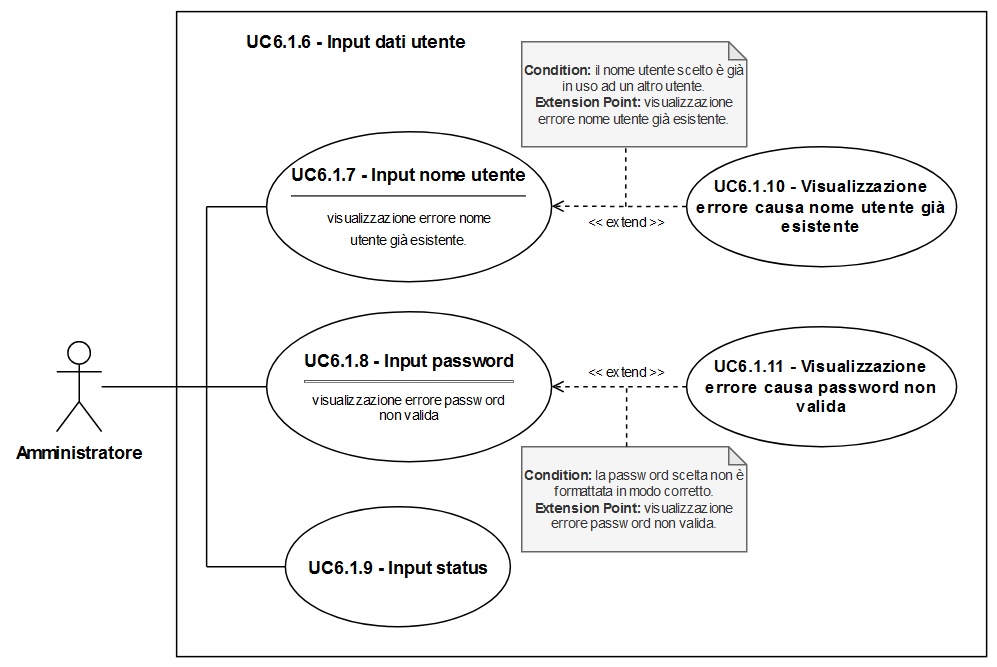
\includegraphics[width=15cm]{images/UC6.1.6.png}
		\caption{Diagramma UC6.1.6 - Input dati utente}
	\end{figure}
	\begin{itemize}
		\item \textbf{Attori primari:} utente amministratore;
		\item \textbf{Descrizione:} l'amministratore inserisce i dati dell'utente interessato;
		\item \textbf{Scenario principale:} 
			\begin{itemize}
				\item l'amministratore esegue l'input del nome utente (UC11.1);
				\item l'amministratore esegue l'input della password (UC11.2);
				\item l'amministratore esegue l'input dello status (UC11.3).
			\end{itemize}
		\item \textbf{Precondizione:} l'amministratore ha accesso all'elenco degli utenti esistenti;
		\item \textbf{Postcondizione:} l'amministratore ha inserito i dati dell'utente interessato.
	\end{itemize}

\subsubsection{UC11.1 - Input nome utente}
	\begin{itemize}
		\item \textbf{Attori primari:} utente amministratore;
		\item \textbf{Descrizione:} l'amministratore inserisce il nome utente da assegnare all'utente interessato;
		\item \textbf{Scenario principale:} l'amministratore esegue l'input del nome utente;
		\item \textbf{Precondizione:} l'amministratore ha accesso all'elenco degli utenti esistenti;
		\item \textbf{Postcondizione:} l'amministratore ha inserito i dati dell'utente interessato.
		\item \textbf{Estensione:}
		\begin{itemize}
			\item \textbf{UC11.4:} se si tenta di usare un nome utente già esistente, viene visualizzato un apposito messaggio di errore.
		\end{itemize}
	\end{itemize}

\subsubsection{UC11.2 - Input password}
	\begin{itemize}
		\item \textbf{Attori primari:} utente amministratore;
		\item \textbf{Descrizione:} l'amministratore inserisce la password da assegnare all'utente interessato;
		\item \textbf{Scenario principale:} l'amministratore esegue l'input della password;
		\item \textbf{Precondizione:} l'amministratore ha accesso all'elenco degli utenti esistenti;
		\item \textbf{Postcondizione:} l'amministratore ha inserito i dati dell'utente interessato.
		\item \textbf{Estensione:}
		\begin{itemize}
			\item \textbf{U11.5:} se si tenta di creare una password che non rispetta le regole di formattazione stabilite, viene visualizzato un apposito messaggio di errore.
		\end{itemize}
	\end{itemize}

\subsubsection{UC11.3 - Input status}
\begin{itemize}
	\item \textbf{Attori primari:} utente amministratore;
	\item \textbf{Descrizione:} l'amministratore sceglie lo status da assegnare all'utente interessato;
	\item \textbf{Scenario principale:} l'amministratore specifica, tra le opzioni disponibili, lo status da assegnare all'utente;
	\item \textbf{Precondizione:} l'amministratore ha accesso all'elenco degli utenti esistenti;
	\item \textbf{Postcondizione:} l'amministratore ha inserito i dati dell'utente interessato.
\end{itemize}

\subsubsection{UC11.4 - Visualizzazione errore causa nome utente già esistente}
	\begin{itemize}
		\item \textbf{Attori primari:} utente amministratore;
		\item \textbf{Descrizione:} l'amministratore visualizza un errore, relativo al fatto che il nome utente che ha tentato di assegnare all'utente è già in uso;
		\item \textbf{Scenario principale:} l'amministratore tenta di inserire un nome utente non valido in quanto assegnato ad un altro utente, ed il sistema risponde con un apposito errore;
		\item \textbf{Precondizione:} l'amministratore ha inserito i dati dell'utente interessato;
		\item \textbf{Postcondizione:} viene visualizzato un errore per informare l'utente che è necessario scegliere un altro nome utente.
	\end{itemize}

\subsubsection{UC11.5 - Visualizzazione errore causa password non valida}
	\begin{itemize}
		\item \textbf{Attori primari:} utente amministratore;
		\item \textbf{Descrizione:} l'amministratore visualizza un errore, relativo al fatto che la password che ha tentato di assegnare all'utente non è valida;
		\item \textbf{Scenario principale:} l'amministratore tenta di inserire una password non valida, ed il sistema risponde con un apposito errore;
		\item \textbf{Precondizione:} l'amministratore sta inserendo i dati dell'utente interessato;
		\item \textbf{Postcondizione:} viene visualizzato un errore per informare l'utente che è necessario scegliere una nuova password.
	\end{itemize}


\subsubsection{UC12 - Visualizzazione mappatura}
	\begin{itemize}
		\item \textbf{Attori primari:} utente amministratore;
		\item \textbf{Descrizione:} l'amministratore prende visione della mappatura dell'ambiente gestito dal sistema;
		\item \textbf{Scenario principale:} l'amministratore visualizza la mappa;
		\item \textbf{Precondizione:} l'amministratore ha accesso alla mappatura dell'ambiente;
		\item \textbf{Postcondizione:} l'amministratore ha visionato la mappatura dell'ambiente.
	\end{itemize}

	\subsubsection{UC13 - Modifica mappatura}
	\begin{itemize}
		\item \textbf{Attori primari:} utente amministratore;
		\item \textbf{Descrizione:} l'amministratore applica le modifiche volute alla mappa;
		\item \textbf{Scenario principale:} l'amministratore formatta la mappa nella maniera voluta;		
		\item \textbf{Precondizione:} l'amministratore ha accesso alla mappatura dell'ambiente;
		\item \textbf{Postcondizione:} l'amministratore ha modificato la mappatura dell'ambiente.
		\item \textbf{Estensione:}
		\begin{itemize}
			\item \textbf{UC11:} se si tenta di formattare la mappa erratamente, viene visualizzato un apposito messaggio di errore.
		\end{itemize}
	\end{itemize}

\subsubsection{UC14 - Visualizzazione errore causa formattazione mappa mal formattata}
	\begin{itemize}
		\item \textbf{Attori primari:} utente amministratore;
		\item \textbf{Descrizione:} l'amministratore visualizza un errore, relativo al fatto che la mappa è stata formattata erratamente;
		\item \textbf{Scenario principale:} l'amministratore tenta di formattare erroneamente la mappa;
		\item \textbf{Precondizione:} l'amministratore sta modificando la mappatura dell'ambiente.
		\item \textbf{Postcondizione:} viene visualizzato un errore per informare l'utente che la mappa è stata mal formattata.
	\end{itemize}


\subsubsection{UC15 - Visualizzazione lista unità}
\begin{itemize}
	\item \textbf{Attori primari:} utente amministratore;
	\item \textbf{Descrizione:} l'amministratore intende prendere visione della lista delle unità presenti nel sistema, e per ognuna viene visualizzato il rispettivo ID;
	\item \textbf{Scenario principale:} l'amministratore visualizza la lista delle unità;
	\item \textbf{Precondizione:} l'amministratore ha accesso all'elenco delle unità esistenti;
	\item \textbf{Postcondizione:} l'amministratore ha visionato la lista delle unità.
\end{itemize}


\subsubsection{UC16 - Inserimento unità}
	\begin{itemize}
		\item \textbf{Attori primari:} utente amministratore;
		\item \textbf{Descrizione:} l'amministratore intende aggiungere una nuova unità, alla lista di quelle gestite dal sistema;
		\item \textbf{Scenario principale:} l'amministratore aggiunge l'unità interessata alla lista di quelle già esistenti fornendo i dati opportuni;
		\item \textbf{Precondizione:} l'amministratore ha accesso all'elenco delle unità esistenti;
		\item \textbf{Postcondizione:} l'amministratore ha modificato la lista delle unità.
		\item \textbf{Inclusione:} 
		\begin{itemize}
			\item \textbf{UC18:} viene eseguito l'input dell'ID dell'unità.
		\end{itemize}
	\end{itemize}

\subsubsection{UC17 - Rimozione unità}
	\begin{itemize}
		\item \textbf{Attori primari:} utente amministratore;
		\item \textbf{Descrizione:} l'amministratore intende eliminare un'unità, dalla lista di quelle gestite dal sistema;
		\item \textbf{Scenario principale:} l'amministratore rimuove l'unità interessata dalla lista di quelle esistenti;
		\item \textbf{Precondizione:} l'amministratore ha accesso all'elenco delle unità esistenti;
		\item \textbf{Postcondizione:} l'amministratore ha modificato la lista delle unità.
	\end{itemize}

\subsubsection{UC18 - Input ID unità}
	\begin{itemize}
		\item \textbf{Attori primari:} utente amministratore;
		\item \textbf{Descrizione:} l'amministratore inserisce l'ID da assegnare all'unità interessata;
		\item \textbf{Scenario principale:} l'amministratore esegue l'input dell'ID unità;
		\item \textbf{Precondizione:} l'amministratore sta inserendo i dati dell'unità interessata;
		\item \textbf{Postcondizione:} l'ID dell'unità risulta inserito;
		\item \textbf{Estensione:}
		\begin{itemize}
			\item \textbf{UC19:} se si tenta di usare l'ID di un'unità già esistente, viene visualizzato un apposito messaggio di errore.
		\end{itemize}
	\end{itemize}

\subsubsection{UC19 - Visualizzazione errore causa ID unità già esistente}
	\begin{itemize}
		\item \textbf{Attori primari:} utente amministratore;
		\item \textbf{Descrizione:} l'amministratore visualizza un errore, relativo al fatto che l'ID che si è cercato di usare è già assegnato ad un'unità esistente;
		\item \textbf{Scenario principale:} l'amministratore tenta di inserire un ID non valido in quanto assegnato ad un'altra unità, ed il sistema risponde con un apposito errore;
		\item \textbf{Precondizione:} l'amministratore sta inserendo i dati dell'unità interessata;
		\item \textbf{Postcondizione:} viene visualizzato un errore per informare l'utente che è necessario scegliere un altro ID per l'unità.
	\end{itemize}